\documentclass{beamer}
\usetheme{metropolis} % Use metropolis theme

\title{ECON 3818: Introduction to Statistics with Computer Applications}
%\subtitle
\date{\today}
\author{Kyle Butts}

\definecolor{blue}{RGB}{0,114,178}
\definecolor{red}{HTML}{EB0E09}
\definecolor{yellow}{RGB}{240,228,66}
\definecolor{green}{RGB}{0,158,115}
\definecolor{maroon}{HTML}{AF3335}
\definecolor{purple}{HTML}{7E90B8}

\definecolor{mybackground}{HTML}{ECECEC}
\setbeamercolor{background canvas}{bg= mybackground}

\definecolor{buff-gold}{HTML}{CFB87C}
\definecolor{buff-grey}{HTML}{565A5C}
\definecolor{buff-lightgrey}{HTML}{A2A4A3}
\definecolor{buff-black}{HTML}{000000}

\setbeamercolor{alerted text}{fg=buff-gold!80!black}
\setbeamercolor{frametitle}{bg=buff-black}
\setbeamercolor{title}{fg=buff-grey}
\setbeamercolor{button}{bg=buff-gold}

% Allow to remove indent w/ \begin{itemize}[leftmargin= *]
\usepackage{enumitem}
\setlist[itemize]{label= \textbullet}

% \usepackage[libertine]{newtxmath}
\usepackage{longtable}
\usepackage{booktabs}
\usepackage{enumitem}


\begin{document}

% Title Page ---------------------------------------
\maketitle


% Chapter 26 ---------------------------------------
\section{Chapter 26: Regression Inference}

\begin{frame}{Introduction}
	
	Chapter 4 and 5 discussed how scatterplots and lines of best fit show us linear relationships, but there are remaining questions

	\begin{itemize}
		\item Is there really a linear relationship between x and y, or is the pattern just by chance
			\begin{itemize}
		      	\item Spurious correlations -- think Nick Cage and number of swimming pool drownings
			\end{itemize}
			  
		\item What is the slope that explains how y responds to x \textit{in the population}, what is the margin of error for that estimate?
		
		\item If we use the least-squares line to predict y for a given x, how accurate is that prediction?
	\end{itemize}
	
\end{frame}

\begin{frame}{Regression Review}
	We can model the linear relationship between X and Y by thinking of a conditional expectation: \[ 
		E(Y|X)= a + bX 
	\]
	
	We want estimates for a and b, $\hat{\alpha}$ and $\hat{\beta}$, and we find these estimates by minimizing the sum of squared residuals
	\[ 
		\varepsilon_i = Y_i - \widehat{Y}_i 
	\]
	where,
	\[ 
		\widehat{Y}_i = \hat{\alpha} +  \hat{\beta} X 
	\]
\end{frame}

\begin{frame}{OLS Estimators}
	Once we minimize the sum of least squares, $\displaystyle\sum_{i=1}^n \varepsilon_i^2 $, we can obtain the Ordinary Least Squares estimators
	
	\[ 
		\hat{\alpha}=\bar{Y}-\hat{\beta}\bar{X} 
	\]
	
	\[ 
		\hat{\beta}=r_{XY}\frac{s_Y}{s_X} 
	\]
\end{frame}

\begin{frame}{Next Steps}
	This chapter will answer

	\begin{itemize}
		\item How can I interpret $\hat{\alpha}$ and $\hat{\beta}$?
		\item Inference from a Regression
		\item What conditions are necessary for those interpretations?
	\end{itemize}

\end{frame}

\begin{frame}{Interpreting $\alpha$ and $\beta$}
	Example: We are studyin a species of coral and how sea surface temperature affects the calcification rate. The equation of the regression line is shown below: \[ 
		\hat{Y}=-12.103+0.4615x 
	\]

	We can now predict how temperature, x, affects the calcification rate, y. The $R^2$ will tell us how much of the variation in calcification rate is due to temperature, but it will not tell us whether this relationship is statistically significant. 
	
	In order for this regression to be meaningful, we must determine whether the results are \alert{statistically significant}
\end{frame}


\begin{frame}{Estimating the Parameters}
	When the conditions for the regression are met:
	
	\begin{itemize}
		\item The slope $\hat{\beta}$ of the least-squares line is an unbiased estimator of the population slope $\beta$
		      
		\item The intercept $\hat{\alpha}$ of the least-squares line is an unbiased estimator of the population intercept $\alpha$
	\end{itemize}
	
	Now we only need to estimate the remaining parameters, $\sigma$
\end{frame}

\begin{frame}{Regression Standard Error}
	Our regression model is: \[ 
		y = \alpha + X \beta + \varepsilon	
	\]
	
	$\varepsilon$ is the error term that describes why an individual doesn't fall directly on regression line $\alpha + X \beta$.

	We denote the variance of $\varepsilon$ as $\sigma^2$. $\sigma$ describes variability of response variable y about the population regression line. 
\end{frame}

\begin{frame}{}
	\begin{itemize}
		\item The least-squares line estimates the population regression line
		\item The \alert{residuals} are the deviations of data points from the least-squares line 
			\[ 
				\hat{\varepsilon} \equiv \text{residual}=\text{observed } y  - \text{predicted } y = y - \hat{y}
			\]
	\end{itemize}

	Therefore we estimate $\sigma$ by the sample standard deviation of the residuals, known as the \alert{regression standard error}
\end{frame}

\begin{frame}{Regression Standard Error}
	\[ 
		s=\sqrt{\frac{1}{n-2}\sum\text{residual}^2}
	\]
	
	\[ 
		s=\sqrt{\frac{1}{n-2}\sum(y-\hat{y})^2}
	\]
	
	We use $s$ to estimate the standard deviation, $\sigma$, of responses about the mean given by the population regression line
	
	We will use this error to determine whether our predictions are statistically significant 
\end{frame}

\begin{frame}{Testing the Hypothesis of No Linear Relationship}
	To answer questions about whether associations between two variables are statistically significant, we must test a hypothesis about the slope $\beta$:
	\begin{align*}
		H_0&: \beta=0 \\
		H_1&: \beta \neq 0 
	\end{align*}

	If we fail to reject $H_0$:
	\begin{itemize}
		\item Regression line with slope 0 is horizontal -- meaning y does not change at all when x changes
		
		\item $H_0$ says that there is no linear relationship between X and Y
	\end{itemize}

	If we reject $H_0$, and accept $H_1$:
	\begin{itemize}
		\item There is some linear relationship between X and Y
	\end{itemize}
\end{frame}

\begin{frame}{Sampling Distribution of $\hat{\beta}$}
	Since $\hat{\beta}$ is a function of our data, it has a sampling distribution.

	The sampling distribution of $\hat{\beta}$ is:
	\[
		\hat{\beta} \sim N\left(\beta, \ \frac{\sigma^2}{\sigma_X^2}\right)
	\]

	$\sigma^2$ is the variance of $\varepsilon$ and $\sigma_X^2$ is the variance of $X$.

	\vspace{5mm}
	\href{https://www.econometrics-with-r.org/4-5-tsdotoe.html}{\beamergotobutton{Visualization of Sampling Distribution}}
	
\end{frame}

\begin{frame}{Significance Test for Regression Slope}
	To test the hypothesis, $H_0: \beta=0$, compute the t-statistic:
	
	\[ 
		t_{n-2}=\frac{\hat{\beta}}{SE_{\hat{\beta}}} 
	\]
	Important to note that the degrees of freedom for the t-statistic for testing a regression slope is $n-2$ 
	
	\vspace{5mm}
	In this formula, the standard error of the least-squares slope is:
	
	\[ 
		SE_{\hat{\beta}}=\frac{s}{\sqrt{\sum (x-\bar{x}^2)}} 
	\]
\end{frame}

\begin{frame}{Example}
	We fit a least-squares line to the model, $\text{Price} = \alpha+\beta (\text{age})$ with 28 observations from items sold at antiques show. A summary of the output is below:

	\begin{center}
		\begin{tabular}{|c|c|c|}
			\hline
			\textbf{Parameter} & \textbf{Parameter Estimate} & \textbf{St. Error of Estimate} \\
			\hline
			$\alpha$  & 27.73 & 34.84 \\
			\hline
			$\beta$   & 1.893 & 0.267 \\
			\hline
		\end{tabular}
	\end{center}

	Suppose we want to test the hypothesis, $H_0: \beta=0$ vs. $H_1: \beta \neq 0$. The value of this t-statistic is: \[ 
		t_{26} = \frac{b}{SE_b} = \frac{1.893}{0.267} = 7.09 
	\]

	Using t-table $\implies p < 0.001$
\end{frame}

\begin{frame}{Clicker Question}
	In the previous example we rejected the null hypothesis of $\beta=0$, meaning we claim there is sufficient evidence to say there is a linear relationship between age and price sold of items at a antiques road show. 
	
	What type of error would we have committed if it turned out there was no relationship between age and price?
	
	\begin{enumerate}[label=(\alph*)]
		\item Type I, reject the null even though its true
		\item Type II, reject the null even though its true
		\item Type I, fail to reject a false null
		\item Type II, fail to reject a false null
	\end{enumerate}
\end{frame}

\begin{frame}{Additional Example -- Exam Style}
	My budtender friend Eric did a study on marijuana consumption and hot cheeto consumption. He surveyed 25 of his friends and collected the following regression results. Assume  $\alpha=0.05$
	
	\begin{center}
		\scalebox{0.9}{
			\begin{tabular}{|c|c|c|c|c|}
				\hline
				\textbf{Cheeto Consumption} & \textbf{Estimate} & \textbf{Std. Error} & \textbf{t-statistic} & \textbf{\ p-value \ } \\
				\hline
				Intercept          & 21       & 12.3       &             &         \\
				\hline
				Joints Smoked      & 4.20     & 1.80       &             &         \\
				\hline
			\end{tabular}
			}
	\end{center}
	\begin{enumerate}[label=(\alph*)]
		\item Fill in the rest of the table
		\item Is the intercept statistically significant? Why?
		\item Is the slope coefficient statistically significant? Why?
		\item Interpret slope coefficient
	\end{enumerate}
\end{frame}


\begin{frame}{Hypothesis Testing Example}
	Example:
	
	Regression analysis provides estimates on the relationship between daily wine consumption on risk of breast cancer. The estimated slope was $\hat{\beta} = 0.009$ with a standard error of $SE_{\hat{\beta}} = 0.001$ based off 25 observations. 
	
	We want to test whether these results are strong enough to reject the null hypothesis $H_0: \beta = 0 $ in favor or the alternative hypothesis $H_1: \beta > 0$
	
	
\end{frame}

\begin{frame}{Hypothesis Testing Example}
	So we have $\hat{\beta}$=0.009 and $SE_{\hat{\beta}}$=0.001.
	Solving hypothesis test:

	\begin{itemize}
		\item Find t-stat \[ 
				t=\frac{0.009}{0.001}=9 
			\]

		\item Use t-table to find p-value \[ 
				25 \text{ observations } \implies t_{n-2} = t_{23} 
			\]
			\[ 
				t_{23}^{0.0005}=3.8 \implies p<0.0005 
			\]

		\item Interpret p-value \[ 
				p<0.0005 \implies p<0.05 \implies \textbf{Reject $H_0$} 
			\]
	\end{itemize}
\end{frame}

\begin{frame}{Regression Results}
	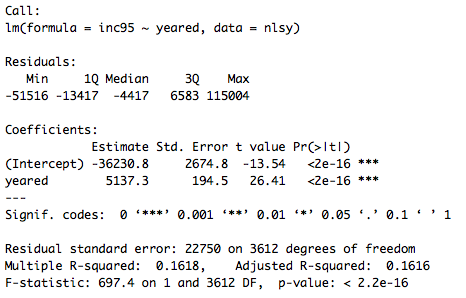
\includegraphics[width=\textwidth]{regression_results}
\end{frame}


\begin{frame}{Confidence Interval for Regression Slope}
	The slope, $\beta$, of the population regression is usually the most important parameter in a regression problem

	\begin{itemize}
		\item The slope is the rate of change of the mean response as the explanatory variable increases
		
		\item The slope explains how changes in x affect outcome variable y
	\end{itemize}
	
	A confidence interval is useful because it shows us \textit{how accurate the estimate of $\beta$ is likely to be}.
\end{frame}




\begin{frame}{Confidence Interval for Regression Slope}
	A level C confidence interval for the slope $\beta$ of the population regression line is
	\[ 
		\hat{\beta} \pm t^* SE_{\hat{\beta}}, \text{ where } t^* = t^{\frac{1-C}{2}}_{n-2}
	\]
\end{frame}




\begin{frame}{Confidence Interval for Regression Slope}
	Example:
	
	Recall our regression results looking at the relationship of temperature on coral calcification. The estimated slope was $\hat{\beta} = 0.4615$ and a standard error $SE_{\hat{\beta}} = 0.07394$. Note this was based off a sample of 12 observations.
	
	If we want to construct a 95\% confidence interval: \[
		\hat{\beta} \pm t^* SE_{\hat{\beta}}= 0.4615 \pm (2.23)(0.07394) 
	\]
	This is because our 12 observations, mean our $t_{n-2}$ distribution has 12-2=10 degrees of freedom and that critical t-stat is 2.23 when $(1-C)/2 = 0.05/2 = 0.025$
	
	The 95\% confidence interval for population slope $\beta$ is $0.297$ to $0.626$.
\end{frame}

\begin{frame}{Clicker Question}
	\small{A random sample of 19 companies were selected and the relationship between sales (in hundreds of thousands of dollars) and profits (in hundreds of thousands of dollars) was investigated by a regression, $profits = \alpha + \beta sales$. The following results were obtained from statistical software:}
	
	\begin{center}
		
			\begin{tabular}{|c|c|c|}
				\hline
				\textbf{Parameter} & \textbf{Parameter Estimate} & \textbf{Std. Error} \\
				\hline
				$\alpha$ & $-176.644$ & $61.16$    \\
				\hline
				$\beta$ & $0.0925$ & $0.0075$   \\
				\hline
			\end{tabular}
		
	\end{center}
	
	\small{ An approximate 90\% confidence interval for the slope $\beta$ is: }

	\begin{enumerate}[label=(\alph*)]
		\item $-176.66$ to $-176.63$
		\item $0.079$ to $0.106$
		\item $0.071$ to $0.114$
	\end{enumerate}
\end{frame}

\begin{frame}{Confidence Intervals}
	Some software programs will automatically spit out a 95\% confidence interval associated with slope estimates, like STATA for example:

	\begin{center}
		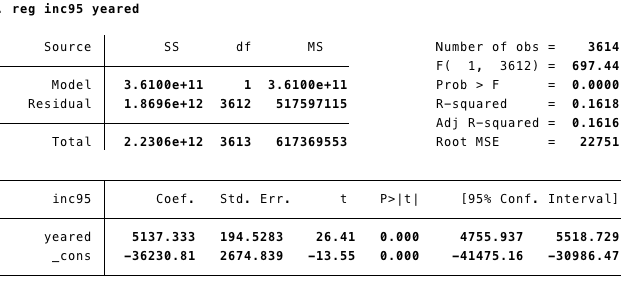
\includegraphics[width=0.9\textwidth]{stata_output}
	\end{center}
	
	95\% confident that an additional year of schooling increases predicted income by \$4,755.9 - \$5,518.7
\end{frame}

\begin{frame}{Significance and Margin of Error}
	\begin{itemize}
		\item Conducting a hypothesis test on $\hat{\beta}$ tells you about the \alert{significance} of your result
			\begin{itemize}
		      	\item p-value $< \alpha$, we can say our coefficient is statistically different from zero
			\end{itemize}

		\item A confidence interval says something about the precision of the coefficient
			\begin{itemize}
		      	\item What are the ranges of coefficient values we expect the true-value to be in between
			\end{itemize}
	\end{itemize}
\end{frame}


\begin{frame}{Significance and Margin of Error}
	
	\begin{center}
		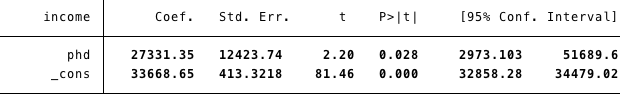
\includegraphics[width=\textwidth]{incphd}
	\end{center}

	\small{
		What we're looking at is the effect of having a PhD on predicted income

		\begin{itemize}
			\item p-value=0.028, which is $<0.05$ (standard $\alpha$)
				\begin{itemize}
			      	\item Enough evidence to overturn null hypothesis that a PhD has no affect on income
				\end{itemize}
			\item Confidence interval = $[2973.1, 51689.6]$
				\begin{itemize}
			      	\item Suggests that the effect of PhD varies greatly. 95\% confident the true mean is between about 3,000 and 50,000. 
				\end{itemize}
		\end{itemize}
	}
\end{frame}

\begin{frame}{Categorical Variable inside Regression}
	In that previous example, the explanatory variable was categorical. Let's see how that changes interpretation.
	
	\begin{center}
		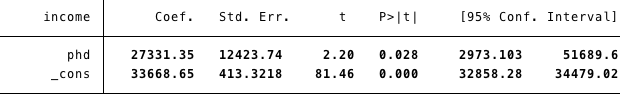
\includegraphics[width=\textwidth]{incphd}
	\end{center}
	
	This regression implies the relationship between PhD and income is: \[ 
		Income = 33,668.65 + 27,331.35 PhD 
	\]
	
	The takeaways here would be:

	\begin{itemize}
		\item Without a PhD, predicted income is \$33,668.65
		\item With a PhD, predicted income is \$33,668.65 + \$27,331.35 = \$61,000
	\end{itemize}
\end{frame}


\begin{frame}{Conditions for Regression Inference}
	Say we have $n$ observations regarding explanatory variable $x$ and response variable $y$. 
	
	\begin{itemize}
		\item The mean response $E(Y|X)$ has a \alert{straight-line relationship} with x, given by a population regression line $$\mu=\alpha+\beta X$$
		
		\item For any fixed value of $x$, the response variable $y$ varies according to a normal distribution
		
		\item Repeated responses $y$ are independent of each other
		
		\item The \alert{standard deviation} of $\varepsilon$, $\sigma$, is the same for all values of x. The value of $\sigma$ is unknown.
	\end{itemize}
\end{frame}



\begin{frame}{Intuition about Conditions}
	\textit{The mean response $E(Y \ \vert \ X)$ has a \alert{straight-line relationship} with x, given by a population regression line}
	
	\begin{itemize}
		\item In practice, we observe y for many different values of x. Eventually we see an overall linear pattern formed by points scattered about the population line. 
	\end{itemize}
\end{frame}

\begin{frame}{Intuition about Conditions}
	\textit{For any fixed value of $x$, the response variable $y$ varies according to a normal distribution}
	
	\begin{itemize}
		\item We cannot observe the entire population regression line. The values of $y$ that we do observe vary about their means according to a normal distribution. If we hold x constant and take many observations of y, the Normal pattern will eventually appear in a histogram. 
	\end{itemize}
\end{frame}

\begin{frame}{Intuition about Conditions}
	\textit{The \alert{standard deviation} of $\varepsilon$, $\sigma$, is the same for all values of x. The value of $\sigma$ is unknown.}
	
	\begin{itemize}
		\item The standard deviation determines whether the points fall close to the population regression line (small $\sigma$) or are widely scattered (large $\sigma$)
			  
		\item If $\sigma$ changes depending on $x$, then our sample distribution would be wrong.
	\end{itemize}
\end{frame}

\begin{frame}{Intuition about Conditions}
	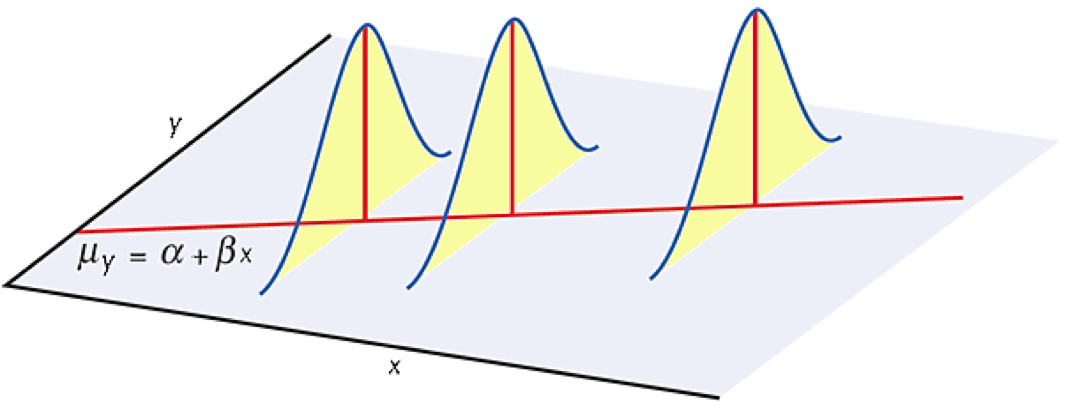
\includegraphics[width=.9\textwidth]{conditions}
	\begin{itemize}
		\item for each possible value of x, the mean of the responses moves along the population regression line
		\item For a fixed x, the responses y follow a normal distribution with std. dev $\sigma$
		      \begin{itemize}
		      	\item value of $\sigma$ determines whether points fall close to the line
		      \end{itemize}
		\item the normal curve shows how y will vary when x is held constant
	\end{itemize}
\end{frame}

\begin{frame}{Checking Conditions for Inference}
	Remember, all of this discussion about inferences hinges on the data meeting certain conditions. 
	\begin{itemize}
		\item The relationship is linear in the population
		\item The response varies normally about the regression line
		\item Observations are independent
		\item The standard deviation of the responses is the same for all values of x
	\end{itemize}
\end{frame}

\begin{frame}{Checking Conditions for Inference}
	In order to check these conditions, it can be helpful to look at a residual plot. A \alert{residual plot} plots the residuals against the explanatory variable x, with a horizontal line at the "residual =0" position. The "residual =0" line represents the position of the least-squares line in the scatterplot of y against x.
	\begin{columns}
		\column{0.5\textwidth}
		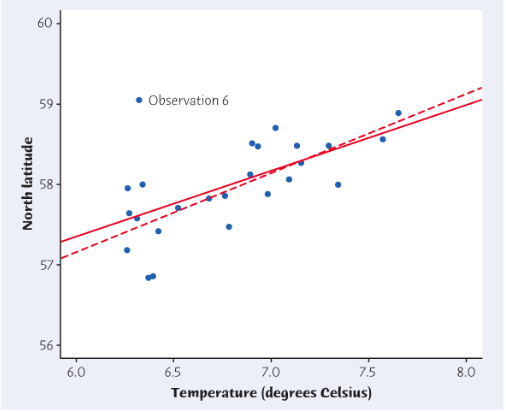
\includegraphics[width=\textwidth]{scatter}
		\column{0.5\textwidth}
		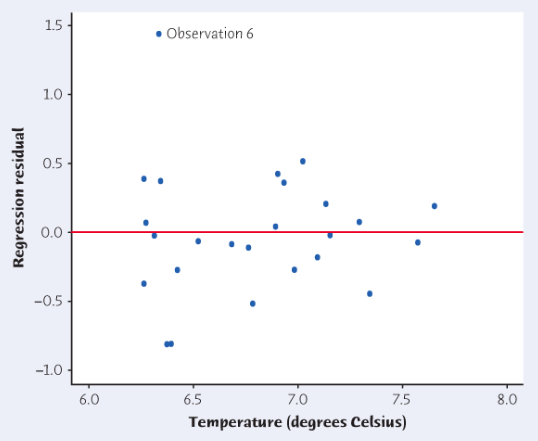
\includegraphics[width=\textwidth]{resid}
	\end{columns}
\end{frame}

\begin{frame}{Checking Conditions for Inference}
	\begin{itemize}
		\item \alert{The relationship is linear}. Look for curved patterns or other deviations from an overall straight line pattern in residual plot
		\item \alert{The response varies normally about regression line}. Check for departures from normality in your stemplot or histogram of residuals.
		\item \alert{Observations are independent}. Signs of dependence in the residual plot are subtle, so usually use common sense. 
		\item \alert{Standard deviation of responses is same for all values of x}. Look at the scatter of residuals above and below the "residual =0" line. The scatter should be roughly the same from one end to the other. 
	\end{itemize}
\end{frame}

\begin{frame}{Residual Histogram}
	\begin{center}
		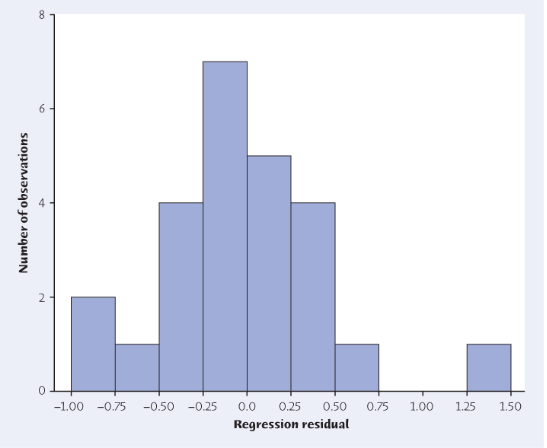
\includegraphics[width=0.75\textwidth]{residual_histo}
	\end{center}
\end{frame}






\end{document}